
\documentclass[fleqn,addpoints]{exam}

\usepackage{graphicx}
\usepackage{booktabs}
\usepackage{float}
\usepackage{amsmath}
\usepackage{cancel}
\usepackage{polynom}
\usepackage{caption}
\usepackage{mdwlist}

\newcommand{\degree}{\ensuremath{^\circ}} 

% \printanswers

\ifprintanswers 
\usepackage{2in1, lscape} 
\fi

\title{Math 115 \\ Homework 27}
\date{June 21, 2011}

\begin{document}

\maketitle

% \begin{figure}[H]
%   \centering
%   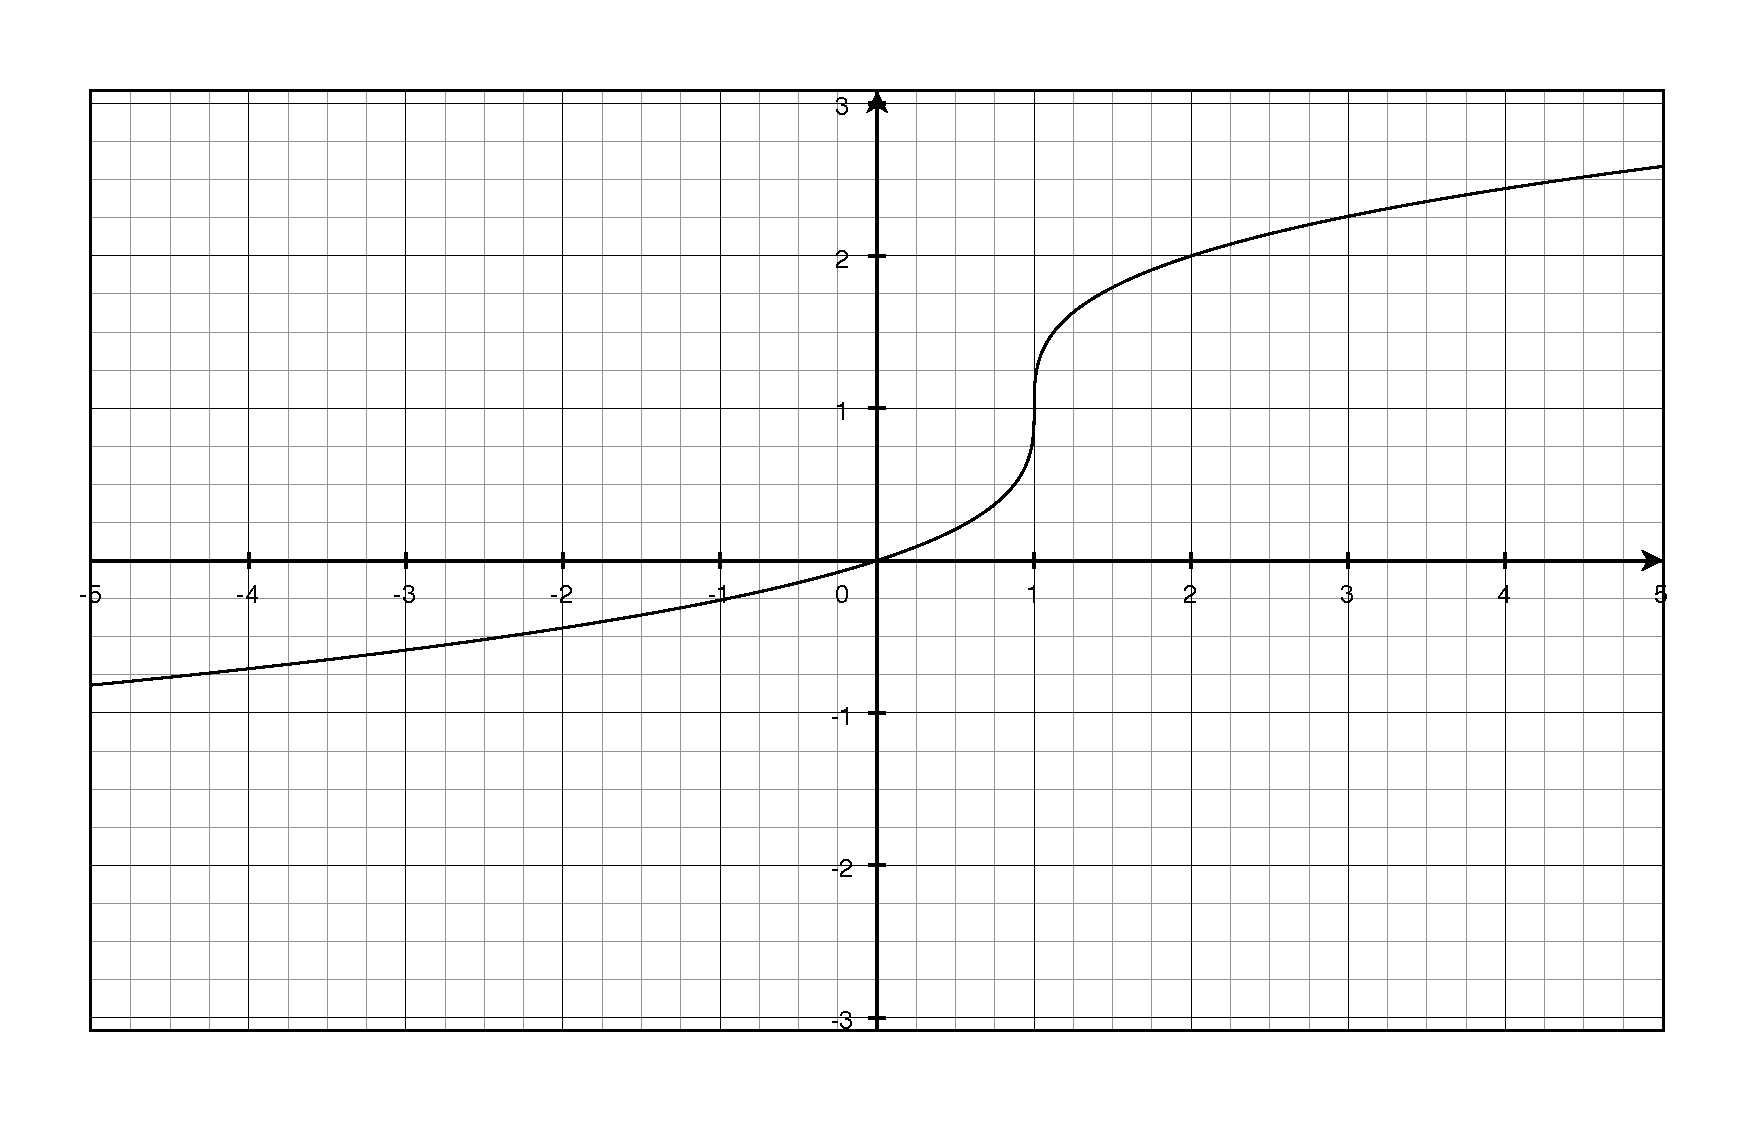
\includegraphics[scale=.3]{question7.eps}
%   \caption*{Question 7}
% \end{figure}

% \begin{tabular}{cc}
% \toprule
% period & amplitude \\
% \midrule
%   $\pi$ & $2$ \\
% \bottomrule
% \end{tabular}

\ifprintanswers
\else

\section{Homework}

Once there was a sultan who wanted all the men in the kingdom to have larger harems.  He thought this would be easy if
he could just manage to increase the number of women, compared to the number of men.  So he came up with the following
law: {\em as soon as a mother gave birth to her first son, she would be forbidden to have any more children}.

In this way, the sultan argued, some families would have several girls and only one boy, but no family could have more
than one boy.  It should not be long until the females would greatly outnumber the males.

Would this law have the desired effect?

\section{Review}

You might want to review some of the things we've covered so far, since it's been a long time since we started in
September.  There are plenty of review problems in the two text books, so take a
look at whatever you feel least comfortable with. 

\vspace{3.5 in}

\begin{em}
Vex not thy spirit at the course of things;  They heed not thy vexation.
\end{em}

\vspace{.2 cm}
\hspace{1.5 cm} --Marcus Aurelius

\fi

\end{document}

